

\arrayrulecolor{Couleur6}

\chapter{Racines carrées et valeurs absolues}




\section{Calculs sur les racines carrées}

\begin{Définition}
La racine carrée d'un nombre réel positif $a$ est l'unique réel positif dont le carré vaut $a$. \\ On la note $\sqrt{a}$ , et on a donc $\sqrt{a}\geq 0$ .
\end{Définition}

\begin{Remarque}
\leavevmode\vspace{-\baselineskip}
\begin{itemize}[label=\textcolor{Couleur7}{$\bullet$}]
\item Par définition, on a $\left(\sqrt{a}\right)^2=a$.
\item $\sqrt{-5}$ n'existe pas ! En effet, il n'existe aucun nombre dont le carré vaut $-5$.
\end{itemize}

\end{Remarque}


\begin{Exemple}
\renewcommand{\arraystretch}{1.3}
\begin{tabular}{>{\centering\arraybackslash}m{2cm}>{\centering\arraybackslash}m{2cm}>{\centering\arraybackslash}m{2cm}>{\centering\arraybackslash}m{2cm}>{\centering\arraybackslash}m{2cm}>{\centering\arraybackslash}m{2cm}>{\centering\arraybackslash}m{2cm}}
 $\sqrt{0}=0$ & $\sqrt{1}=1$ & $\sqrt{4}=2$ & $\sqrt{9}=3$ & $\sqrt{16}=4$ & $\sqrt{25}=5$ & $\sqrt{36}=6$  \\
$\sqrt{49}=7$ & $\sqrt{64}=8$ & $\sqrt{81}=9$ & $\sqrt{100}=10$ & $\sqrt{121}=11$ & $\sqrt{144}=12$ & $\sqrt{169}=13$
\end{tabular}

\end{Exemple}

\begin{Remarque}
$\sqrt{2}\approx 1,4142$ et $\sqrt{3}\approx 1,732$ sont des nombres irrationnels.

\end{Remarque}

\vspace{0.4cm}

\begin{Propriété}
Pour tous réels positifs $a$ et $b$, on a $\sqrt{ab}=\sqrt{a}\sqrt{b}$.
\end{Propriété}

\begin{proof}
D'une part, $\left(\sqrt{a}\times \sqrt{b}\right)^2=\left(\sqrt{a}\right)^2\times \left(\sqrt{b}\right)^2=a\times b$ par définition de la racine carrée ($a$ et $b$ positifs).\\
D'autre part, $\left(\sqrt{a\times b}\right)^2=a\times b$ par définition de la racine carrée ($a$ et $b$ positifs, donc $a\times b$ aussi).\\
Donc, $\left(\sqrt{a}\times \sqrt{b}\right)^2=\left(\sqrt{a\times b}\right)^2$. \\
Or, $\sqrt{a}\times \sqrt{b}$ et $\sqrt{a\times b}$ sont positifs et de carrés égaux, ils sont donc égaux.\\ Ainsi, $\sqrt{ab}=\sqrt{a}\sqrt{b}$.

\end{proof}
\vspace{-0,5cm}
\begin{Exemple}
Réduire au maximum les nombres suivants :
\begin{itemize}[label=\textcolor{Couleur8}{$\bullet$}]
\item $\sqrt{98}=\sqrt{49\times 2}=\sqrt{49}\times \sqrt{2}=7\sqrt{2}$.
\item $2\sqrt{2}\times 4\sqrt{18}=8\sqrt{2\times 18}=8\sqrt{36}=8\times 6=48$.
\item $\left(4\sqrt{5}\right)^2=4^2\times\left(\sqrt{5}\right)^2=16\times 5=80$.
\item $3\sqrt{125}=3\times \sqrt{25\times 5}=3\times 5\sqrt{5}=15\sqrt{5}$.
\end{itemize}

\end{Exemple}


\begin{Propriété}
Pour tous réels positifs $a$ et $b$ avec $b\neq 0$, on a $\sqrt{\dfrac{a}{b}}=\dfrac{\sqrt{a}}{\sqrt{b}}$.
\end{Propriété}



\begin{Exemple}
\leavevmode\vspace{-\baselineskip}
\begin{multicols}{2}
\begin{itemize}[label=\textcolor{Couleur8}{$\bullet$}]
\item $\dfrac{\sqrt{32}\times\sqrt{10}}{\sqrt{80}}=\sqrt{\dfrac{32\times 10}{80}}=\sqrt{4}=2$.
\item $\sqrt{\dfrac{50}{242}}=\sqrt{\dfrac{25}{121}}=\dfrac{\sqrt{25}}{\sqrt{121}}=\dfrac{5}{11}$.
\end{itemize}
\end{multicols}
\end{Exemple}

\newpage

\begin{Méthode}Simplifier une écriture contenant des racines carrées. \\

\begin{enumerate}
\item Écrire le plus simplement possible : 
\begin{itemize}[label=\textcolor{Couleur3}{$\bullet$}]
\item $A=4\sqrt{3}-2\sqrt{3}+6\sqrt{3}$
\item $B=(3-2\sqrt{5})-(4-6\sqrt{5})$
\end{itemize}


\item Écrire les expressions suivantes sous la forme $a\sqrt{b}$, où $a$ et $b$ sont des entiers et $b$ le plus petit possible :
\begin{itemize}[label=\textcolor{Couleur3}{$\bullet$}]
\item $C=\sqrt{12}+7\sqrt{3}-\sqrt{27}$
\item $D=\sqrt{125}-2\sqrt{20}+6\sqrt{80}$
\end{itemize}
\item Écrire les expressions suivantes sous la forme $\dfrac{a\sqrt{b}}{c}$, où $a$, $b$ et $c$ sont des entiers et $b$ le plus petit possible :
\begin{itemize}[label=\textcolor{Couleur3}{$\bullet$}]

\item $E=\dfrac{-5}{\sqrt{2}}$
\item $F=\dfrac{1}{3+\sqrt{5}}$

\end{itemize}
\end{enumerate}


\begin{enumerate}
\item 

$A=4\sqrt{3}-2\sqrt{3}+6\sqrt{3}=(4-2+6)\sqrt{3}=8\sqrt{3}$.\\
$B=(3-2\sqrt{5})-(4-6\sqrt{5})=3-2\sqrt{5}-4+6\sqrt{5}=-1+4\sqrt{5}$.

\item 

$C=\sqrt{12}+7\sqrt{3}-\sqrt{27}=\sqrt{4\times 3}+7\sqrt{3}-\sqrt{9\times 3}=2\sqrt{ 3}+7\sqrt{3}-3\sqrt{ 3}=6\sqrt{3}$.\\
$D=\sqrt{125}-2\sqrt{20}+6\sqrt{80}=\sqrt{25\times 5}-2\sqrt{4\times 5}+6\sqrt{16\times 5}=5\sqrt{5}-4\sqrt{5}+24\sqrt{5}=25\sqrt{5}$.

\item 

$E=\dfrac{-5}{\sqrt{2}}=\dfrac{-5\times \sqrt{2}}{\sqrt{2}\times \sqrt{2}}=\dfrac{-5\times \sqrt{2}}{2}$. \\

$F=\dfrac{1}{3+\sqrt{5}}=\dfrac{1\times (3-\sqrt{5})}{(3+\sqrt{5})\times (3-\sqrt{5})}=\dfrac{3-\sqrt{5}}{9+3\sqrt{5}-3\sqrt{5}+\sqrt{5}\times \sqrt{5}}=\dfrac{3-\sqrt{5}}{9+5}=\dfrac{3-\sqrt{5}}{14}$.
\end{enumerate}


\end{Méthode}

\begin{Propriété}
Pour tous réels $a$ et $b$ strictement positifs, on a $\sqrt{a+b} < \sqrt{a} +\sqrt{b}$.

\end{Propriété}

\begin{proof}
Comme $a$ et $b$ sont strictement positifs, $\sqrt{a+b}$ et $ \sqrt{a} +\sqrt{b}$ sont positifs. \\
Donc montrer que $\sqrt{a+b} < \sqrt{a} +\sqrt{b}$, revient à montrer que $\left(\sqrt{a+b}\right)^2 < \left(\sqrt{a} +\sqrt{b}\right)^2$. \\
C'est à dire, montrer que $\left(\sqrt{a+b}\right)^2 -\left(\sqrt{a} +\sqrt{b}\right)^2 <0$. 
\begin{align*}
\left(\sqrt{a+b}\right)^2 -\left(\sqrt{a} +\sqrt{b}\right)^2 &= a+b -(a+2\sqrt{a}\sqrt{b}+b) \\
&=a+b -a-2\sqrt{a}\sqrt{b}-b \\
&=-2\sqrt{a}\sqrt{b}\\
\end{align*}
Or, $\sqrt{a}>0$ et $\sqrt{b}>0$ car $a$ et $b$ sont strictement positifs. Donc, $-2\sqrt{a}\sqrt{b}<0$.\\
Finalement, $\left(\sqrt{a+b}\right)^2 -\left(\sqrt{a} +\sqrt{b}\right)^2 <0$ et donc $\sqrt{a+b} < \sqrt{a} +\sqrt{b}$.


\end{proof}



\newpage

\section{La fonction racine carrée}
\subsection{Définition, représentation graphique et propriété}

\begin{Définition}
La fonction racine carrée est la fonction définie sur $[0;+\infty[$ par $f:x\mapsto \sqrt{x}$.

\end{Définition}

\begin{center}

\begin{tabular}{|c|c|c|c|c|c|c|c|}
\hline
$x$ & $0$ & $0,25$ & $1$ & $2,25$ & $4$ & $6,25$ & $9$ \\
\hline
$f(x)=\sqrt{x}$ & $0$ & $0,5$ & $1$ & $1,5$ & $2$ & $2,5$ & $3$ \\
\hline

\end{tabular}
\end{center}

 \begin{center}
\begin{tikzpicture}[x=1.4cm,y=1.2cm]
% Définition des limites
\def\xmin{-0.5}
\def\xmax{10.5}
\def\ymin{-0.5}
\def\ymax{4.5}

% Grille en pointillés
\draw[dotted, gray] (0,0) grid[step=0.5] (10.5,4.5);

% Axes
\draw[->,thick] (\xmin,0) -- (\xmax,0) node[below right] {$x$};
\draw[->,thick] (0,\ymin) -- (0,\ymax) node[above left] {$y$};

% Graduations sur l'axe x
\foreach \x in {0.5,1,1.5,2,2.5,3,3.5,4,4.5,5,5.5,6,6.5,7,7.5,8,8.5,9,9.5,10}
    \draw (\x,2pt) -- (\x,-2pt) node[below] {\x};

% Graduations sur l'axe y
\foreach \y in {0.5,1,1.5,2,2.5,3,3.5,4}
    \draw (2pt,\y) -- (-2pt,\y) node[left] {\y};

% Origine
\draw (0,0) node[below left] {0};

% Courbe y = sqrt(x)
\draw[samples=300,domain=0:10.5,Couleur6,thick] plot (\x,{sqrt(\x)});

% Label de la fonction
\draw[Couleur6] (9.5,3.8) node {$y=\sqrt{x}$};



% Points sur la courbe (croix noires)
\draw[thick] (0,0) node {$\times$};
\draw[thick] (0.25,0.5) node {$\times$};
\draw[thick] (1,1) node {$\times$};
\draw[thick] (2.25,1.5) node {$\times$};
\draw[thick] (4,2) node {$\times$};
\draw[thick] (6.25,2.5) node {$\times$};
\draw[thick] (9,3) node {$\times$};

\end{tikzpicture}
\end{center}

\begin{Propriété}
La fonction racine carrée est croissante sur $[0;+\infty[$.

\end{Propriété}

\noindent On peut donc dresser le tableau de variation de la fonction racine carrée. 
\begin{center}
  \begin{tikzpicture}
      \tkzTabInit[espcl=5,lgt=3]{$x$ / 1, Variations de $f(x)=\sqrt{x}$ /2 } { $0$  , $+\infty$ };
\tkzTabVar{ -/$0$ ,  +/ };
      \end{tikzpicture} 
      \end{center}
      
      
 \begin{proof}
 Soient $a$ et $b$ deux réels positifs distincts tels que $a< b$.\\
 On veut montrer que $f(a)<f(b)$, c'est-à-dire que $\sqrt{a}<\sqrt{b}$. Cela revient à montrer que $\sqrt{a}-\sqrt{b}<0$. \\
 \begin{align*}
 \sqrt{a}-\sqrt{b} &= \dfrac{(\sqrt{a}-\sqrt{b})(\sqrt{a}+\sqrt{b})}{\sqrt{a}+\sqrt{b}} \\
 &= \dfrac{a-b}{\sqrt{a}+\sqrt{b}}
 \end{align*}
 Or, comme $a$ et $b$ sont positifs et différents, $\sqrt{a}+\sqrt{b}>0$ et $a-b>0$ car $a<b$. \\
 Ainsi, $\sqrt{a}<\sqrt{b}$.\\
 $a$ et $b$ étant deux réels quelconques de $]0;+\infty[$, la fonction racine carrée est croissante sur $]0;+\infty[$.
 \end{proof}
 
 \newpage
 \subsection{Équations et inéquations}
 
 \begin{minipage}[c]{0.68\linewidth}
 \begin{Propriété}
Pour tout réel $a$, l'équation $\sqrt{x}=a$ admet pour ensemble de solutions :
\begin{itemize}[label=\textcolor{Couleur2}{$\bullet$}]
\item $S=\{a^2\}$ si $a\geq 0$
\item $S=\emptyset$ si $a<0$.
\end{itemize}

\end{Propriété}
\begin{Exemple}
L'équation $\sqrt{x}=3$ a pour ensemble de solutions $S=\{9\}$.
\end{Exemple}
 \end{minipage} \hfill
 \begin{minipage}[c]{0.25\linewidth}
\begin{center}
\begin{tikzpicture}[x=0.7cm,y=0.7cm]
% Définition des limites
\def\xmin{-1}
\def\xmax{5}
\def\ymin{-0.9}
\def\ymax{4}

% Grille en pointillés
\draw[dotted, gray] (0,0) grid[step=1] (5,4);

% Axes
\draw[->,thick] (\xmin,0) -- (\xmax,0) node[below right] {$x$};
\draw[->,thick] (0,\ymin) -- (0,\ymax) node[above left] {$y$};

% Origine
\draw (0,0) node[below left] {0};

% Graduations principales
\foreach \x in {1}
    \draw (\x,2pt) -- (\x,-2pt) node[below] {$\x$};

\foreach \y in {1}
    \draw (2pt,\y) -- (-2pt,\y) node[left] {$\y$};

% Courbe y = sqrt(x)
\draw[samples=300,domain=0:5,Couleur6,thick] plot (\x,{sqrt(\x)});

% Lignes en pointillés Couleur3 pour montrer la relation a et a²
\draw[dashed,Couleur10,thick] (0,1.6) node[left] {$a$} -- (2.56,1.6) -- (2.56,0) node[below] {$a^2$};

\end{tikzpicture}
\end{center}
 \end{minipage}







\begin{minipage}[c]{0.68\linewidth}
\begin{Propriété}
Pour tout réel $a$, l'inéquation $\sqrt{x}\leq a$ admet pour ensemble de solutions :
\begin{itemize}[label=\textcolor{Couleur2}{$\bullet$}]
\item $S=[0;a^2]$ si $a\geq 0$
\item $S=\emptyset$ si $a<0$.
\end{itemize}
Pour tout réel $a$, l'inéquation $\sqrt{x}\geq a$ admet pour ensemble de solutions :
\begin{itemize}[label=\textcolor{Couleur2}{$\bullet$}]
\item $S=[a^2;+\infty[$ si $a\geq 0$
\item $S=[0;+\infty[$ si $a<0$.
\end{itemize}
\end{Propriété}
\begin{Exemple}
\leavevmode\vspace{-\baselineskip}
\begin{itemize}[label=\textcolor{Couleur8}{$\bullet$}]
\item L'inéquation $\sqrt{x}\leq 4$ a pour ensemble de solutions $S=[0;16]$.
\item L'inéquation $\sqrt{x}>5$ a pour ensemble de solutions $S=]25;+\infty[$.
\item L'inéquation $-4\sqrt{x}-5<7$ qui s'écrit aussi $\sqrt{x}>-3$ a pour ensemble de solutions $S=]0;+\infty[$.
\end{itemize}

\end{Exemple}

\end{minipage} \hfill
\begin{minipage}[c]{0.25\linewidth}
\begin{center}
\begin{tikzpicture}[x=0.7cm,y=0.7cm]
% Définition des limites
\def\xmin{-1}
\def\xmax{5}
\def\ymin{-0.9}
\def\ymax{4}

% Ligne épaisse rose sur l'axe x (de 0 à a²)
\draw[line width=4pt, Couleur6!45!white] (0,0) -- (2.56,0);

% Grille en pointillés
\draw[dotted, gray] (0,0) grid[step=1] (5,4);

% Axes
\draw[->,thick] (\xmin,0) -- (\xmax,0) node[below right] {$x$};
\draw[->,thick] (0,\ymin) -- (0,\ymax) node[above left] {$y$};

% Origine
\draw (0,0) node[below left] {0};

% Graduations principales
\foreach \x in {1}
    \draw (\x,2pt) -- (\x,-2pt) node[below] {$\x$};

\foreach \y in {1}
    \draw (2pt,\y) -- (-2pt,\y) node[left] {$\y$};

% Courbe y = sqrt(x) en deux parties
% Partie rose : de 0 à a² (où sqrt(x) ≤ a)
\draw[samples=300,domain=0:2.56,Couleur6,thick] plot (\x,{sqrt(\x)});

% Partie verte : de a² à 5 (où sqrt(x) > a)
\draw[samples=300,domain=2.56:5,Couleur3,thick] plot (\x,{sqrt(\x)});

% Label pour la condition
\draw[Couleur6] (2,3.5) node {$\sqrt{x}\leq a$};

% Lignes en pointillés Couleur3 pour montrer la relation a et a²
\draw[dashed,Couleur10,thick] (0,1.6) node[left] {$a$} -- (2.56,1.6) -- (2.56,0) node[below] {$a^2$};

\end{tikzpicture}
\end{center}
~\\
\begin{center}
\begin{tikzpicture}[x=0.7cm,y=0.7cm]
% Définition des limites
\def\xmin{-1}
\def\xmax{5}
\def\ymin{-0.9}
\def\ymax{4}

% Ligne épaisse rose sur l'axe x (de 0 à a²)
\draw[line width=4pt, Couleur6!45!white] (2.56,0) -- (5,0);

% Grille en pointillés
\draw[dotted, gray] (0,0) grid[step=1] (5,4);

% Axes
\draw[->,thick] (\xmin,0) -- (\xmax,0) node[below right] {$x$};
\draw[->,thick] (0,\ymin) -- (0,\ymax) node[above left] {$y$};

% Origine
\draw (0,0) node[below left] {0};

% Graduations principales
\foreach \x in {1}
    \draw (\x,2pt) -- (\x,-2pt) node[below] {$\x$};

\foreach \y in {1}
    \draw (2pt,\y) -- (-2pt,\y) node[left] {$\y$};

% Courbe y = sqrt(x) en deux parties
% Partie rose : de 0 à a² (où sqrt(x) ≤ a)
\draw[samples=300,domain=0:2.56,Couleur3,thick] plot (\x,{sqrt(\x)});

% Partie verte : de a² à 5 (où sqrt(x) > a)
\draw[samples=300,domain=2.56:5,Couleur6,thick] plot (\x,{sqrt(\x)});

% Label pour la condition
\draw[Couleur6] (2,3.5) node {$\sqrt{x}\geq a$};

% Lignes en pointillés Couleur3 pour montrer la relation a et a²
\draw[dashed,Couleur10,thick] (0,1.6) node[left] {$a$} -- (2.56,1.6) -- (2.56,0) node[below] {$a^2$};

\end{tikzpicture}
\end{center}
\end{minipage}





\vspace{-0,5cm}

\section{Valeur absolue et distance entre deux réels}
\subsection{Valeur absolue d'un nombre réel}
\begin{Définition}
Soit $x$ un nombre réel.\\
On appelle valeur absolue de $x$, notée $\vert x \vert$, le nombre égal à $\left\{
    \begin{array}{ll}
         x & \text{ si } x\geq 0 \\
        -x & \text{ si } x\leq 0 
    \end{array}
\right.$

\end{Définition}

\begin{Exemple}
\renewcommand{\arraystretch}{1.3}
\begin{tabular}{>{\centering\arraybackslash}m{3cm}>{\centering\arraybackslash}m{6cm}>{\centering\arraybackslash}m{6cm}}
 $\vert 24 \vert =24$
& $\vert -19,2 \vert =19,2$
& $\vert x-5 \vert =\left\{
    \begin{array}{ll}
        x-5  & \text{ si } x\geq 5\\
        5-x &  \text{ si } x\leq 5
    \end{array}
\right.$ 
\end{tabular}
\end{Exemple}

\begin{Remarque}
Pour un réel $x$, on a : $\vert -x \vert =\vert x \vert$.
\end{Remarque}

\begin{Propriété}
Pour tout réel $x$, $\sqrt{x^2}=\vert x\vert $
\end{Propriété}

\begin{Exemple}
\begin{multicols}{3}
\vspace{-0.5cm}
$\sqrt{(5,1)^2}=5,1$
\\
$\sqrt{ (-2)^2} =2$\\
$\sqrt{(12-2x)^2}=\vert 12-2x \vert =\left\{
    \begin{array}{ll}
        12-2x  & \text{ si } x\leq 6\\
        2x-12 &  \text{ si } x\geq 6
    \end{array}
\right.$

\end{multicols}
\vspace{-0.5cm}
\end{Exemple}




\newpage

\subsection{Distance entre deux réels}

\begin{Définition}
Soit $a$ et $b$ deux nombres réels.\\
On appelle distance entre $a$ et $b$ le nombre $\vert a-b \vert$.

\end{Définition}

\begin{Exemple}
La distance entre $-3$ et $7$ est $\vert -3 -7\vert =\vert -10\vert =10$.
\end{Exemple}

\begin{Propriété}
Soient $a$ et $r$ deux réels avec $r \geq 0$.\\
L'intervalle $\intff{a-r}{a+r}$ est l'ensemble des réels $x$ tels que $\vert x-a \vert \leq r$.

\end{Propriété}

\begin{Exemple}
Soit un réel $x$ tel que $\vert x-8 \vert \leq 3$. Cela signifie que $x\in \intff{8-3}{8+3}=\intff{5}{11}$.\\
Sur une droite graduée, cela veut dire que la distance du point d'abscisse $x$ au point d'abscisse $8$ est inférieure ou égale à $3$.

\end{Exemple}
\begin{center}
\begin{tikzpicture}[x=2cm]

% Axe horizontal avec flèche
\draw[thick,->] (4,0) -- (12,0);

% Graduations sur l'axe
\foreach \x in {5,6,7,8,9,10,11}
    \draw[very thick] (\x,2pt) -- (\x,-2pt) node[below] {\small\x};

% Points importants
\draw[Couleur6] (5.7,0) node {$\bullet$};
\draw[Couleur3] (5,0) node {$\bullet$};
\draw[Couleur3] (11,0) node {$\bullet$};

% Label pour x
\draw (5.7,0) node[below] {$x$};

% Arcs verts montrant les distances de 3 unités
\draw[thick,>=stealth,->,Couleur10] (8,0) to[bend right] (5,0.2);
\draw[thick,>=stealth,->,Couleur10] (8,0) to[bend left] (11,0.2);

% Labels "3" sur les arcs
\draw[Couleur10] (6.5,1.5) node {$3$};
\draw[Couleur10] (9.5,1.5) node {$3$};

% Flèche rose montrant l'intervalle solution
\draw[<->,Couleur6] (5.7,-1) -- (8,-1);

% Label de l'inégalité
\draw[Couleur6] (6.8,-1) node[below] {$\vert x-8 \vert \leq 3$};

\end{tikzpicture}
\end{center}

\bigskip

\newpage

\section*{Exercices - Racines carrées et valeurs absolues}
\addcontentsline{toc}{section}{Exercices}
{\setlength{\columnseprule}{0pt}
\setcounter{NumEx}{1}


\subsection*{Racine carrée}
\begin{Exercice}
Simplifier au maximum les expressions suivantes :
\vspace{-0.5cm}
\begin{multicols}{4}
\begin{enumerate}
    \item $A = \sqrt{16}$
    \item $B = \sqrt{8}$
    \item $C = \sqrt{18}$
    \item $D = \dfrac{81}{49}$
    \item $E = \sqrt{6} \sqrt{2}$
    \item $F = \sqrt{6} \times \sqrt{7} \sqrt{3}$
    \item $G = \sqrt{27} \times \sqrt{8} \sqrt{24}$
    \item $H = (\sqrt{5})^4$
\end{enumerate}
\end{multicols}
\end{Exercice}

\begin{Exercice}
Développer et réduire au maximum les expressions suivantes :
\vspace{-0.5cm}
\begin{multicols}{2}
\begin{enumerate}
    \item $A = \left( \sqrt{5} + \sqrt{3} \right)  ^2$
    \item $B = \left( 1 - \sqrt{2})(1 + \sqrt{2} \right) $
    \item $C = \left( 3 + \sqrt{8})(4 + \sqrt{2} \right) $
    \item $D = \left( \sqrt{12} - \sqrt{27} \right) ^2$
\end{enumerate}
\end{multicols}
\end{Exercice}

\begin{Exercice}
Simplifier au maximum l’expression $A = 2\sqrt{20} - \sqrt{45} + \sqrt{125}$.
\end{Exercice}



% @see : https://coopmaths.fr/alea?uuid=12b72&id=2N32-4&n=4&d=10&s=1&alea=FxVx&cd=1&cols=2
\begin{Exercice}
\leavevmode\vspace{-\baselineskip}
\vspace{-0.5cm}
\begin{multicols}{2}
\begin{enumerate}[itemsep=1em]
	\item \begin{minipage}[t]{\linewidth} Écrire $A=-4\sqrt{891} -5\sqrt{275} +7\sqrt{396}$ sous la forme $a\sqrt{11}$ où $a$ est un entier. \end{minipage}
	\item \begin{minipage}[t]{\linewidth} Écrire $B=7\sqrt{539} +3\sqrt{99} -7\sqrt{44}$ sous la forme $a\sqrt{11}$ où $a$ est un entier. \end{minipage}
	\item \begin{minipage}[t]{\linewidth} Écrire $C=8\sqrt{54} -7\sqrt{600} -2\sqrt{96}$ sous la forme $a\sqrt{6}$ où $a$ est un entier. \end{minipage}
	\item \begin{minipage}[t]{\linewidth} Écrire $D=-6\sqrt{726} +3\sqrt{24} +7\sqrt{150}$ sous la forme $a\sqrt{6}$ où $a$ est un entier. \end{minipage}
\end{enumerate}
\end{multicols}
\end{Exercice}

% @see : https://coopmaths.fr/alea?uuid=d9495&id=2N32-3&n=4&d=10&s=1&alea=eEIe&cd=1&cols=2
\begin{Exercice}
\leavevmode\vspace{-\baselineskip}
\vspace{-0.5cm}
\begin{multicols}{2}
\begin{enumerate}[itemsep=1em]
	\item \begin{minipage}[t]{\linewidth} Écrire $\sqrt{486}$ sous la forme $a\sqrt{6}$ où $a$ est un entier. \end{minipage}
	\item \begin{minipage}[t]{\linewidth} Écrire $\sqrt{150}$ sous la forme $a\sqrt{6}$ où $a$ est un entier. \end{minipage}
	\item \begin{minipage}[t]{\linewidth} Écrire $\sqrt{125}$ sous la forme $a\sqrt{5}$ où $a$ est un entier. \end{minipage}
	\item \begin{minipage}[t]{\linewidth} Écrire $\sqrt{12}$ sous la forme $a\sqrt{3}$ où $a$ est un entier. \end{minipage}
\end{enumerate}
\end{multicols}
\end{Exercice}

% @see : https://coopmaths.fr/alea?uuid=99b29&id=2N32-2&n=6&d=10&s=1&alea=OSDT&cd=1&cols=3
\begin{Exercice}
Donner, si possible, une écriture simplifiée des calculs suivants.
\begin{multicols}{3}
\begin{enumerate}[itemsep=1em]
	\item \begin{minipage}[t]{\linewidth} $ 3 \sqrt{7}\left( 4  +3\sqrt{7}\right)$ \end{minipage}
	\item \begin{minipage}[t]{\linewidth} $\left(-8 \sqrt{10}\right)^{2}$ \end{minipage}
	\item \begin{minipage}[t]{\linewidth} $ \sqrt{30}\times \sqrt{5}$ \end{minipage}
	\item \begin{minipage}[t]{\linewidth} $\sqrt{7}+\sqrt{2}$ \end{minipage}
	\item \begin{minipage}[t]{\linewidth} $ \sqrt{\dfrac{294}{6}}$ \end{minipage}
	\item \begin{minipage}[t]{\linewidth} $  \sqrt{4}+\sqrt{16}$ \end{minipage}
\end{enumerate}
\end{multicols}
\end{Exercice}

\begin{Exercice}
On appelle nombre d’or, noté $\phi$, le réel $\phi = \dfrac{1 + \sqrt{5}}{2}$. Montrer que multiplier $\phi$ par lui-même revient à lui ajouter 1.
\end{Exercice}

\begin{Exercice}
On considère un triangle $ABC$ tel que $AB = 4\sqrt{3}$, $BC = 2\sqrt{12}$ et $CA = 4\sqrt{6}$. Quelle est la nature du triangle $ABC$ ?
\end{Exercice}

% @see : https://coopmaths.fr/alea?uuid=4771d&id=2N32-7&n=3&d=10&s=1&alea=vfkA&cd=1&cols=3
\begin{Exercice}Trouver une fraction égale à celle proposée en supprimant la racine carrée de son dénominateur.
\begin{multicols}{3}
\begin{enumerate}[itemsep=1em,label={}]
	\item \begin{minipage}[t]{\linewidth} $A=\dfrac{ 5 }{\sqrt{10}} $ \end{minipage}
	\item \begin{minipage}[t]{\linewidth} $B=\dfrac{ 2 }{\sqrt{10}} $ \end{minipage}
	\item \begin{minipage}[t]{\linewidth} $C=\dfrac{ 11 }{\sqrt{2}} $ \end{minipage}
\end{enumerate}
\end{multicols}
\end{Exercice}

% @see : https://coopmaths.fr/alea?uuid=4771d&id=2N32-7&n=3&d=10&s=2&alea=u2ld&cd=1&cols=4
\begin{Exercice}
Trouver une fraction égale à celle proposée en supprimant la racine carrée de son dénominateur.
\begin{multicols}{4}
\begin{enumerate}[itemsep=1em,label={}]
	\item \begin{minipage}[t]{\linewidth} $A=\dfrac{ 4 }{6+4\sqrt{3}} $  \end{minipage}
	\item \begin{minipage}[t]{\linewidth} $B=\dfrac{ 3 }{3-6\sqrt{10}} $  \end{minipage}
	\item \begin{minipage}[t]{\linewidth} $C=\dfrac{ 5 }{6-3\sqrt{10}} $  \end{minipage}
\end{enumerate}
\end{multicols}
\end{Exercice}

\begin{Exercice}
Écrire les expressions suivantes sous la forme $a + b\sqrt{c}$.
\vspace{-0.5cm}
\begin{multicols}{3}
\begin{enumerate}
    \item $\dfrac{3}{1 + \sqrt{2}}$
    \item $\dfrac{4}{2 - 3\sqrt{5}}$
    \item $\dfrac{1 + \sqrt{3}}{2 + \sqrt{7}}$
\end{enumerate}
\end{multicols}
\end{Exercice}

\begin{Exercice}
Montrer que $\sqrt{2 + \sqrt{3}} = \dfrac{\sqrt{6} + \sqrt{2}}{2}$.
\end{Exercice}

\begin{Exercice}
Déterminer les domaines de définitions des fonctions suivantes.
\vspace{-0.5cm}
\begin{multicols}{2}
\begin{enumerate}
    \item $f : x \mapsto \sqrt{x - 5}$
    \item $g : x \mapsto \sqrt{x^2 + 3}$
    \item $h : x \mapsto \sqrt{9 - x}$
    \item $i : x \mapsto \sqrt{(2x - 6)(-3x + 12)}$
\end{enumerate}
\end{multicols}
\end{Exercice}

\newpage

\begin{Exercice}
Tom doit résoudre l'équation $ \sqrt{x-1} = 5 $. Voici sa résolution :
« On pose $ X = x-1 $.
\begin{align*}
 \sqrt{x-1} = 5 &\Leftrightarrow \sqrt{X}=5 \\
 &\Leftrightarrow X=25\\
 &\Leftrightarrow x-1=25\\
 &\Leftrightarrow x=26
 \end{align*}
 $ S=\left\lbrace 26 \right\rbrace  $\\
 
À la manière de Tom, résoudre l'équation $ \sqrt{x+3} = 12 $.
\end{Exercice}

\begin{Exercice}
Lilia doit résoudre l'inéquation $ \sqrt{2x+1} \leq 5 $. Voici sa résolution :
« On pose $ X = 2x-1 $.
\begin{align*}
 \sqrt{2x-1} \leq 5 &\Leftrightarrow \sqrt{X} \leq 5 \\
 &\Leftrightarrow 0 \leq X \leq 25\\
 &\Leftrightarrow 0 \leq 2x+1 \leq 25\\
 &\Leftrightarrow -1 \leq 2x \leq 24\\
  &\Leftrightarrow -\dfrac{1}{2} \leq x \leq 12
 \end{align*}
 $ S=\left[ -\dfrac{1}{2}; 12\right]   $\\
 
À la manière de Lilia, résoudre l'équation $ \sqrt{x-3} \geq 7 $.
\end{Exercice}

\begin{Exercice}
La vitesse d'un tsunami dépend de la profondeur de l'océan dans lequel il se propage. Cette vitesse y (en $ km.h^{-1} $) se calcule par la formule : $ v=870\sqrt{\dfrac{h}{6}} $ où $ h $ est la profondeur de l'océan (en km).
\begin{enumerate}
\item Quelle est la vitesse d'un tsunami qui se propage dans un océan de 6 km de profondeur ?
\item Quelle est la profondeur de l'océan lorsque
$ V = 1000 km.h^{-1} $ ? Arrondir au km près.
\item On a tracé la fonction $ v $ dans le repère ci-dessous.
\begin{center}
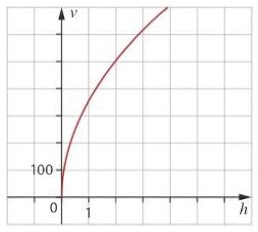
\includegraphics[scale=1]{Ch 11/Ex11}
\end{center}
Déterminer l'intervalle des profondeurs telles que la vitesse $ v $ soit inférieure ou égale à $500 km.h^{-1}$
\end{enumerate}
\end{Exercice}
\newpage
\begin{Exercice}
Lorsqu'un bateau se présente en amont d'une écluse, il faut faire monter le niveau de l'eau afin que le bateau puisse rejoindre l'aval de l'écluse (voir figure ci-après).
\begin{center}
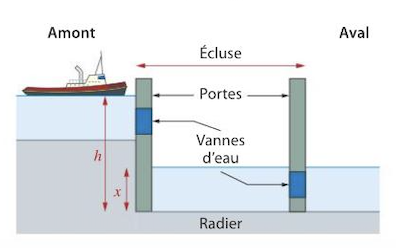
\includegraphics[scale=1]{Ch 11/Ex12}
\end{center}
On note $ h $ (en mètres) la hauteur du niveau de l'eau en amont de l'écluse et $ x $ la hauteur (en mètres) du niveau de l'eau dans l'écluse. Ces hauteurs sont mesurées à partir du fond de l'écluse appelé le radier.\\
Un bateau se présente lorsque $ h = 5,2 m $ et $ x = 2,1 m $.
À cet instant, on ouvre les vannes pour remplir l'écluse.
La vitesse v d'écoulement de l'eau (en $ m.s^{-1} $) versée par les vannes a pour expression : $ v=\sqrt{2g(h-x)} $
où $ g = 9,8 m.s^{-2} $ est l'accélération de la pesanteur.
\begin{enumerate}
\item Calculer la vitesse de l'eau au moment où le bateau se présente en amont de l'écluse. Arrondir au dixième.
\item Pour quelle valeur de $ x $ la vitesse d'écoulement de l'eau est-elle nulle ?
\item \begin{enumerate}
\item Tracer dans le repère ci-dessous la courbe représentative de la fonction $ x \mapsto v(x) $, avec $ h = 5,2 m $.
\begin{center}
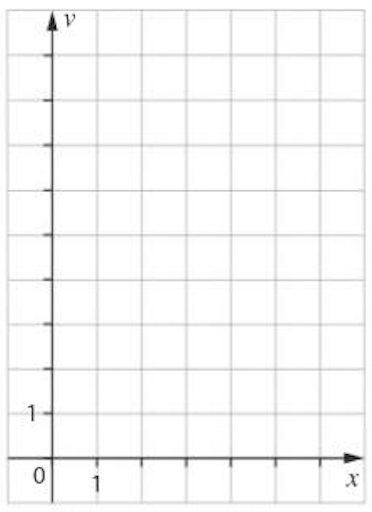
\includegraphics[scale=.7]{Ch 11/Ex12q3}
\end{center}
\item  Déterminer graphiquement la hauteur $ x $ de l'eau dans l'écluse lorsque $ v = 5 m.s^{-1} $.
\item  Retrouver ce résultat par le calcul.
\end{enumerate}
\end{enumerate}
\end{Exercice}

\newpage

\subsection*{Valeur absolue}

\begin{Exercice}
Dans chacun des cas suivants, donner la valeur absolue $|x - y|$.
\vspace{-0.5cm}
\begin{multicols}{3}
\begin{enumerate}
    \item $x = 1$ et $y = 3$
    \item $x = 5$ et $y = -1$
    \item $x = \dfrac{1}{2}$ et $y = \dfrac{1}{3}$
\end{enumerate}
\end{multicols}
\end{Exercice}

\begin{Exercice}
Effectuer les calculs suivants sans utiliser la calculatrice
\begin{enumerate}
    \item $A = 2 \times |1 - 4| - 5 \times |7 - 3| + |5 - (-1)| \times |-2 - 3|$
    \item $B = \dfrac{2}{3} \times \left| \dfrac{1}{4} - \dfrac{1}{3} \right| + \dfrac{1}{4} \times \left| \dfrac{1}{2} - \dfrac{1}{5} \right|$
\end{enumerate}
\end{Exercice}

\begin{Exercice}
Dans chacun des cas suivants, déterminer les valeurs des réels $x$ vérifiant les égalités suivantes.
\vspace{-0.5cm}
\begin{multicols}{3}
\begin{enumerate}
    \item $|x| = 8$
    \item $|x - 2| = 5$
    \item $|x - 7| = 4$
    \item $|x + 1| = 2$
    \item $|x + 7| = 3$
    \item $|x + 4| = -2$
\end{enumerate}
\end{multicols}
\end{Exercice}

\begin{Exercice}
Déterminer le(s) réel(s) $x$ vérifiant $|x - 3| = |x + 1|$.
\end{Exercice}

\begin{Exercice}
Dans chacun des cas suivants, déterminer les valeurs des réels $x$ vérifiant les égalités suivantes.
\vspace{-0.5cm}
\begin{multicols}{3}
\begin{enumerate}
    \item $|2x + 1| = 7$
    \item $|3 - x| = 8$
    \item $|5 - 2x| = 1$
\end{enumerate}
\end{multicols}
\end{Exercice}

\begin{Exercice}
Soit $x$ un réel. Exprimer les inégalités suivantes en termes d'intervalle.
\vspace{-0.5cm}
\begin{multicols}{3}
\begin{enumerate}
    \item $|x| \leq 7$
    \item $|x| < 4$
    \item $|x - 2| \leq 3$
    \item $|x - 4| < 19$
    \item $|x + 20| \leq 31$
    \item $|x + 4| < 1$
\end{enumerate}
\end{multicols}
\end{Exercice}

\begin{Exercice}
Traduire chacun des intervalles suivants à l'aide d'une inégalité de la forme $|x - a| \leq b$ ou $|x - a| < b$.
\vspace{-0.5cm}
\begin{multicols}{3}
\begin{enumerate}
    \item $[3 ; 9]$
    \item $]-1 ; 5[$
    \item $[-2 ; 0]$
    \item $[10 ; 19]$
    \item $]-5 ; 12[$
    \item $[\dfrac{5}{2} ; 10]$
\end{enumerate}
\end{multicols}
\end{Exercice}


}
